\documentclass[12pt, a4paper, oneside, british]{report}
\usepackage{epigraph}
\usepackage{setspace}
\usepackage[dvipsnames]{xcolor}
\usepackage[british]{babel}
\usepackage{amssymb}
\usepackage{amsmath}
\usepackage{pgfplotstable}
\usepackage{pgfplots}
\usepackage{natbib}
\usepackage[hyphens]{url}
\bibliographystyle{abbrvnat}

%Diagramme
\usepackage{pgfplots}
\usepackage{pgfplotstable}

\usepackage[singlelinecheck=false,font={footnotesize, it}, tablewithin=section,
figurewithin=section,format=hang]{caption}

\usepackage{multirow}
\usepackage{footnote}
\makesavenoteenv{tabular}
%To Use Float Barrier
\usepackage{placeins}

%For Listings
\usepackage{listings}
\usepackage{lstlinebgrd}
% DOS-Fontstyle
\newenvironment{DOS_Font}{\footnotesize\color{black}\rmfamily}{\par}

\lstdefinestyle{DOS}
{
    backgroundcolor=\color{white},
    basicstyle=\footnotesize\color{black}\rmfamily,
    breaklines = true,
    breakatwhitespace=true,
    captionpos=rb
}

\lstdefinestyle{DOSScriptsize}
{
    backgroundcolor=\color{white},
    basicstyle=\footnotesize\color{black}\rmfamily,
    breaklines = true,
    breakatwhitespace=true,
    captionpos=rb
}

\lstdefinestyle{Wireshark}
{
    backgroundcolor=\color{white},
    basicstyle=\footnotesize\color{black}\rmfamily,
    captionpos=rb,
    breaklines=true,
    breakatwhitespace=true,
    tabsize=1,
    frame=single
}

\lstdefinestyle{WiresharkTiny}
{
    backgroundcolor=\color{white},
    basicstyle=\tiny\color{black}\rmfamily,
    captionpos=rb,
    breaklines=true,
    breakatwhitespace=true,
    tabsize=1,
    frame=single
}

\lstdefinestyle{WiresharkScriptSize}
{
    backgroundcolor=\color{white},
    basicstyle=\scriptsize\color{black}\rmfamily,
    captionpos=rb,
    breaklines=true,
    breakatwhitespace=true,
    tabsize=1,
    frame=single
}

%For Abbreviations
\usepackage[printonlyused]{acronym}

%For Headers and Footers
\usepackage{fancyhdr}
\renewcommand{\chaptermark}[1]{\markboth{#1}{}}
\renewcommand{\sectionmark}[1]{\markright{\arabic{section}.\ #1}}

\pagestyle{fancy}
\fancyhf{}
%\rhead{\itshape\nouppercase{\leftmark}} %shows chapter
\rhead{\itshape\nouppercase{\rightmark}}
\lfoot{Workshop \courseNumber - Acquistapace, Just, Lesnianski,
Schneider}
\rfoot{\thepage}
\renewcommand{\headrulewidth}{1pt}
\renewcommand{\footrulewidth}{1pt}

\newcommand{\prof}{Dionysios Satikidis, MSc }
\newcommand{\courseNumber}{7 }
\newcommand{\courseName}{Embedded Systems Engineering }
\newcommand{\teamNo}{B}
\newcommand{\teamName}{SmartCart}
\newcommand{\assignmentName}{IoT Applications Prototyping }
\newcommand{\assignmentAuthorOne}{Timo Acquistapace }
\newcommand{\studentNumberOne}{1644604 }
\newcommand{\assignmentAuthorTwo}{Markus Just }
\newcommand{\studentNumberTwo}{1644609 }
\newcommand{\assignmentAuthorThree}{Wojciech Lesnianski }
\newcommand{\studentNumberThree}{1644612 }
\newcommand{\assignmentAuthorFour}{Simon Schneider }
\newcommand{\studentNumberFour}{xxx }
\begin{document}
\onehalfspacing
\setlength\epigraphrule{0pt}
\setlength{\epigraphwidth}{0.8\textwidth}
\renewcommand{\epigraphflush}{flushleft}

\bibliography{resources}
\begin{titlepage}
	\flushright
	
\includegraphics[width=0.50\textwidth]{res/Brunel_University_Logo.png}\par
	\centering
	\line(1,0){390}\\
	\vfill
	\raggedright
	{\scshape Workshop \courseNumber: \par}
	{\Huge\bfseries \courseName\par}
	{\Large\bfseries \assignmentName\par}
	\vspace{1.5cm}
	
	\begin{tabular}{lll}
	Team \teamNo: & \multicolumn{2}{l}{\teamName} \\
	Date:	& \multicolumn{2}{l}{\today} \\
	Lecturer: & \multicolumn{2}{l}{\prof} \\
	& & \\
	& & \\
	Team members: & & \\
	\hline
	Project leader: & \studentNumberOne & \assignmentAuthorOne \\
	Developer: & \studentNumberThree & \assignmentAuthorThree \\
	Data-Analyst: & \studentNumberTwo & \assignmentAuthorTwo \\
	Documentation-Manager: & \studentNumberFour & \assignmentAuthorFour \\
	& & \\
	Deadline & 24\textsuperscript{th} April, 2017
	\end{tabular}
		
	\vfill
	\line(1,0){390}
	\flushleft
% Bottom of the page
\end{titlepage}
\pagenumbering{gobble}

\tableofcontents 
\newpage
% \begin{raggedleft}
% \begin{huge}
% \textbf{List of Abbreviations}
% \end{huge}
% \end{raggedleft}

\section*{List of Abbreviations}

\begin{acronym}[abcdefghijklmno]
 \input{contents/abbreviations.txt}
\end{acronym}
%\setcounter{chapter}{2}
\setcounter{page}{1}
\pagenumbering{arabic}

\begin{abstract}
I think I spider, we should write one page of abstract!
\end{abstract}

\chapter{Smart Cart - A smarter Way of Shopping}

In the following sections, the idea and implementation of SmartCart -- an
Android application that will simplify your shopping experience -- will be
exposed. The application was created in the course of the workshop
``\assignmentName'' by the team IoT-Designers:

\begin{table}[h]
\renewcommand\arraystretch{1}
\centering
\begin{tabular}{p{0.21\textwidth}p{0.21\textwidth}p{0.21\textwidth}p{0.21\textwidth}}
\begin{center}Timo\end{center} & 
\begin{center}Wojciech\end{center} & 
\begin{center}Markus\end{center} & 
\begin{center}Simon\end{center}
\\
\vspace{-1.25cm}\begin{center}Acquistapace\end{center} & 
\vspace{-1.25cm}\begin{center}Lesnianski\end{center} & 
\vspace{-1.25cm}\begin{center}Just\end{center} & 
\vspace{-1.25cm}\begin{center}Schneider\end{center}
\\
\vspace{-1cm}\begin{center}
\includegraphics[width=0.2\textwidth]{res/intro/Timo.png}\end{center}
& 
\vspace{-1cm}\begin{center}
\includegraphics[width=0.2\textwidth]{res/intro/Ich.png}\end{center}
&
\vspace{-1cm}\begin{center}
\includegraphics[width=0.2\textwidth]{res/intro/Markus.png}\end{center}
&
\vspace{-1cm}\begin{center}
\includegraphics[width=0.2\textwidth]{res/intro/Simon.png}\end{center}
\\
\vspace{-1cm}\begin{center}Project Leader\end{center} & 
\vspace{-1cm}\begin{center}Developer\end{center} & 
\vspace{-1cm}\begin{center}Data Analyst\end{center} &
\vspace{-1cm}\begin{center}Documentation Manager \end{center}
\end{tabular}
\end{table}

\section{Introduction}
Since the idea of SmartCart evolved during the workshop, this section firstly
introduces the initial product idea of SmartCart and the change of scope that
project went through. Later on, the architecture and the system's context
as well as the used state machine and its evolution are described. The following
sections focus on the recognition of gestures. For this purpose, the
mathematical basics that are necessary to recognize gestures are derived and the
gestures that are used to control the system are introduced.

\subsection{Initial Idea of SmartCart}
The first concept of SmartCart was to offer its user the possibility to add
items to a shopping list and to get this shopping list ordered automatically as
the user enters a supermarket. The entered grocery is determined with the help
of the Microsoft Here API. Based on the knowledge of the accessed shop and the
ordering of its departments, the items that were previously added to the shopping list,
should be ordered.

\subsection{Change of Scope and final Idea of SmartCart}
Even though the initial idea of SmartCart would have been a very helpful
application to the user, it is strongly based on the collaboration with the
operators of the supported supermarkets. This is especially true for the data
acquisition regarding the offered products and the available departments of a
supermarket. Therefore, the initial scope of the application was changed towards
an application that is less dependent on master data.

The revised concept of SmartCart focusses more on the interaction of the user
and the application. It omits the features of recognising a shop that is entered
and ordering the list of shopping items according to the recognised shop.
Instead, the application should offer the possibility of easily marking an item
as �added to the cart� and of navigating through the list via gestures. The
recognition of gestures is done via the built-in sensors for acceleration and
the magnetic field sensor.

Even the initial idea was discarded during the workshop for the mentioned
reasons, the focus that is now put on the user interaction might nevertheless
support the initial idea. 

\section{System Analysis}
The upfront steps that were taken to create a shared understanding and to
examine possible solutions in building the application are shortly presented in
the current section.

\subsection{Determination of the Use Cases}
SmartCart in its final scope addresses two main use cases: the use case of
creating a shopping list and adding items to it as well as the process of going
shopping itself. The use case ``Go shopping�� implements the main user
interaction that consists of switching to the previous / next item and of
marking an item of the shopping list as �added to cart�. This interaction takes
place via gestures made by the user with its smartphone and detected by the
SmartCart application.

\begin{figure}
\centering
\captionsetup{justification=centering}
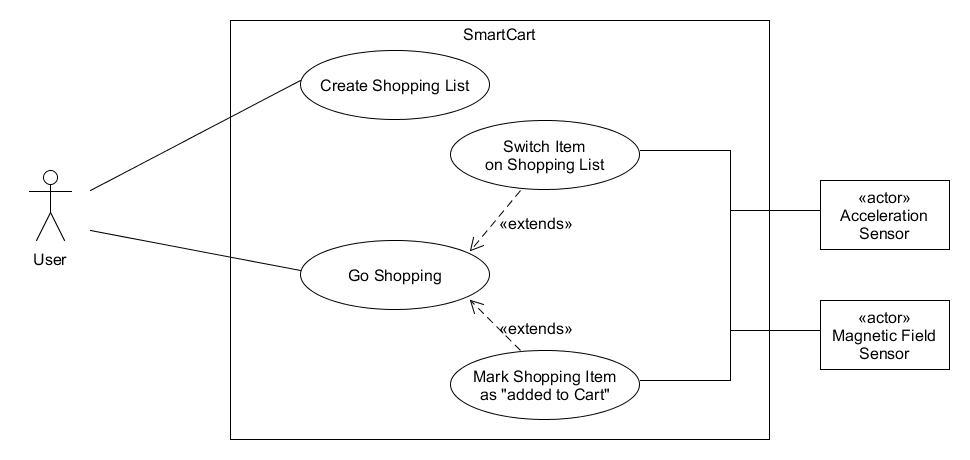
\includegraphics[width=\textwidth]{res/sa/useCaseDiagram.png}
\caption{Overview of the System's Use Cases}
\label{fig:UseCases}
\end{figure}

\subsection{Relations between the captured Gestures
and the used Sensors}

\begin{figure}
\centering
\captionsetup{justification=centering}
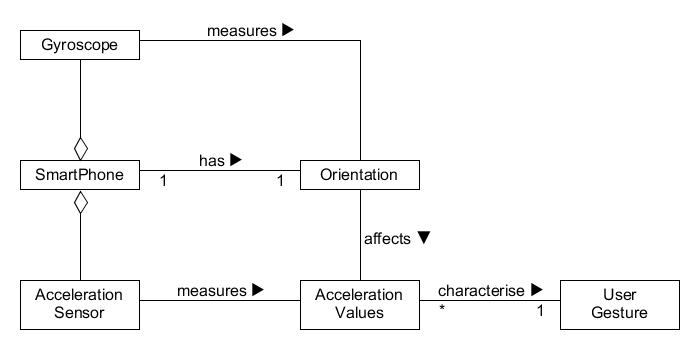
\includegraphics[width=\textwidth]{res/sa/UserGestureDataModel.png}
\caption{Data Model of the User Gestures to recognize}
\label{fig:UseCases}
\end{figure}

\section{Data Acquisition and Data Analysis}
\label{sect:dataAnalysis}

\listoftables
\listoffigures
\bibliography{resources} 

\end{document}
